
\begin{figure}[h]
  \centering
  \begin{tabular}{ p{3cm} p{0.7cm} p{4cm} p{0.7cm} p{4cm} }
    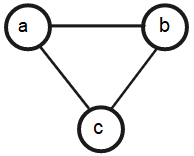
\includegraphics[width=2.3cm]{./img/trianguloabc} && 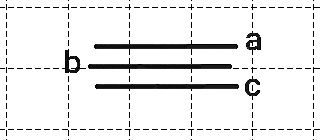
\includegraphics[width=3.9cm]{./img/b0epgTransparenciaGrade2} & &
    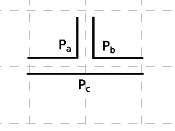
\includegraphics[width=3.5cm]{./img/b1EpgTransparenteGrade2}
    \\
    \footnotesize
    (a) The  graph $C_3$. && \footnotesize(b) $B_0$-EPG representation of $C_3$ (edge-clique).&& \footnotesize(c) $B_1$-EPG representation of $C_3$ (claw-clique).\\
  \end{tabular}

 \caption{The  graph $ C_3 $  and  representations without bends and with 1 bend.} \label{fig:trianguloepgRepresentacao}
\end{figure}
